\chapter{Przetwornik C/A}

\section{Treść zadania}
\begin{itemize}
    \item Należało zmontować \textbf{sumator o trzech wejściach} korzystając z \textbf{licznika modulo 8} oraz \textbf{wzmacniacza operacyjnego} o zadanym schemacie:
        \begin{figure}[H]
            \centering
            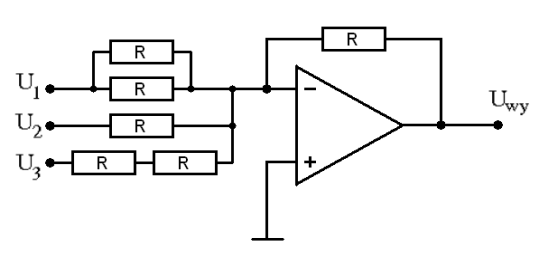
\includegraphics[width=0.7\textwidth]{img/schemes/2.png}
            \caption{Schemat układu sumatora}
            \label{fig:my_label}
        \end{figure}
    \item Napięcia \textbf{U1}, \textbf{U2}, \textbf{U3} zostawały podawane z licznika modulo 8, gdzie \textbf{LSB} (least significant bit) podpięty został do napięcia \textbf{U1}.
\end{itemize}

\section{Budowa licznika modulo 8}

\begin{itemize}
    \item Licznik modulo 8 zbudowano za pomocą układu JK 7493.
        \begin{figure}[H]
            \centering
            \begin{subfigure}[H]{0.35\textwidth}
                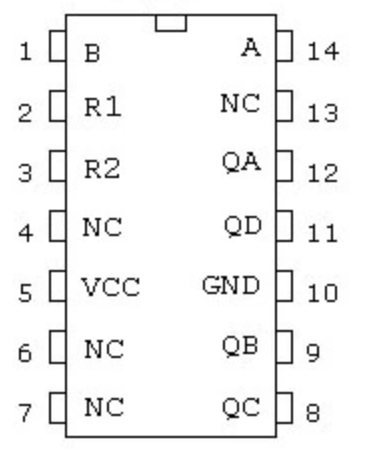
\includegraphics[width=\textwidth]{img/schemes/7493_pins.png}
                \caption{Piny TTL 7493}
            \end{subfigure}
            \begin{subfigure}[H]{0.6\textwidth}
                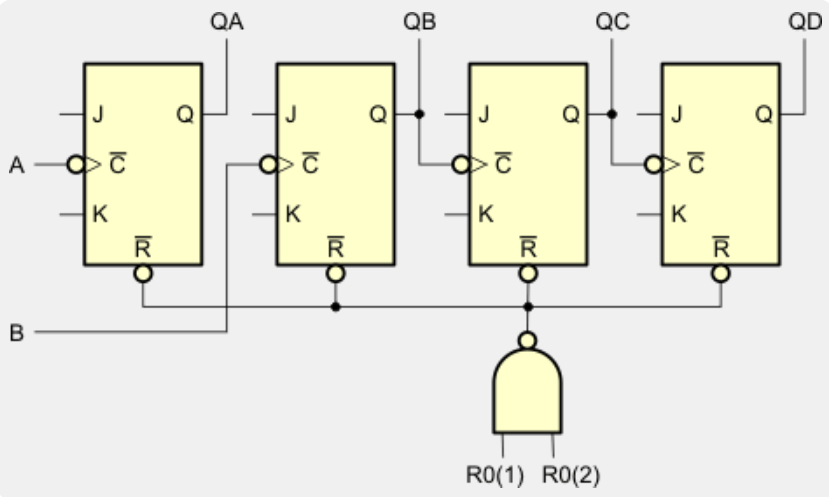
\includegraphics[width=\textwidth]{img/schemes/logic_scheme_7943.png}
                \caption{Schemat logiczny 7493}
            \end{subfigure}
            \label{licznik_mod16:piny_schemat_logiczny}
        \end{figure}
    \item Do wejścia B (pin 1) wpięto sygnał z generatora funkcyjnego o wartościach:
        \begin{center}
            f = 1Hz \\
            $U_{low}$ = 0V \\
            $U_{high}$ = 5V
        \end{center}
    \item Oba wejścia resetu wpięto pod impulsator (wciśnięcie impulsatora resetuje licznik do pozycji w której każdy bit = 0).
    \item Wyjścia licznika (QB, QC, QD) zostały wyprowadzone do diod elektroluminescencyjnych     znajdujących się na prawej stronie płytki.
    \item LSB (least significant bit) podpięty jest pod pierwszą diodę od lewej (wyjście QB).
        \begin{figure}[H]
            \centering
            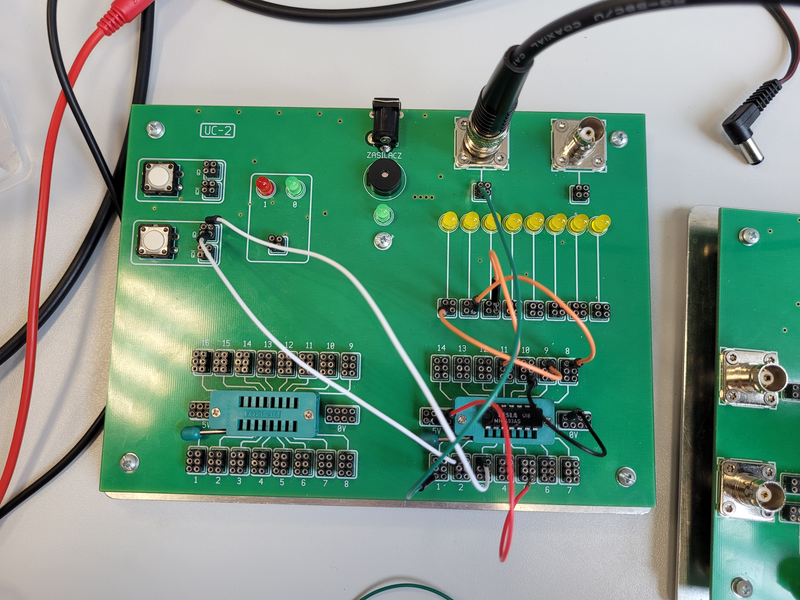
\includegraphics[width=0.7\textwidth]{img/2/20220608_092500_scaled.png}
            \caption{Zbudowany licznik mod 8}
            \label{licznik_mod8:zbudowany_uklad}
        \end{figure}
        
        \begin{figure}[H]
            \centering
            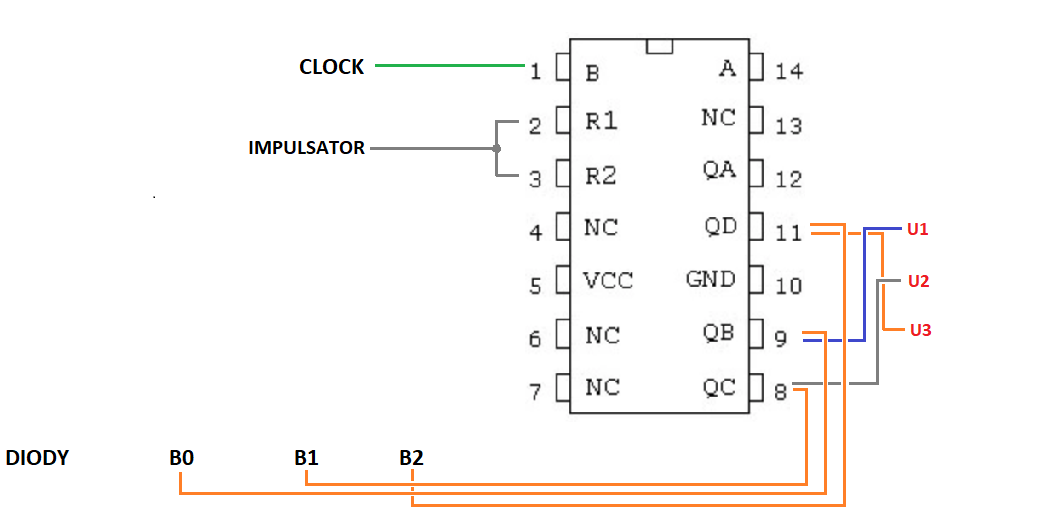
\includegraphics[width=0.9\textwidth]{img/schemes/schemat_w_pins.png}
            \caption{Schemat z połączonymi pinami}
        \end{figure}
        
    \item Licznik działał \textbf{poprawnie}. Po sekwencji $(111)_2 = (7)_{10}$ licznik resetował stan do $(000)_2 = (0)_{10}$. Wciśnięcie impulsatora powodowało reset aktualnego stanu licznika do stanu wyzerowanego $(000)_2$.
\end{itemize}

\section{Dodanie wzmacniacza operacyjnego}

\begin{itemize}
    \item Do płytki ze wzmacniaczem doprowadzono napięcia U1, U2, U3 z wejść kolejno: QB, QC, QD.
    \item Korzystając ze schematu układu dobrano rezystory:
        Teoretyczne wartości korzystając z łączenia rezystorów ($R_1$ - równoległe, $R_3$ - szeregowe):
        \begin{gather}
            R_1 = \dfrac{R}{2} \\
            R_2 = R \\
            R_3 = 2R
        \end{gather}
        \begin{equation}
            -5V = -R_f * 5V(\dfrac{1}{\frac{R}{2}}+\dfrac{1}{R}+\dfrac{1}{2R}) \implies R_f = \dfrac{2}{7}R
        \end{equation}
        Dobrane rezystory (zmierzone multimetrem):
        \begin{gather}
            R_1 = 1.48k\Omega \\
            R_2 = 2.71k\Omega \\
            R_3 = 5.56k\Omega \\
            R_f = 813\Omega
        \end{gather}
        \begin{figure}[H]
            \centering
            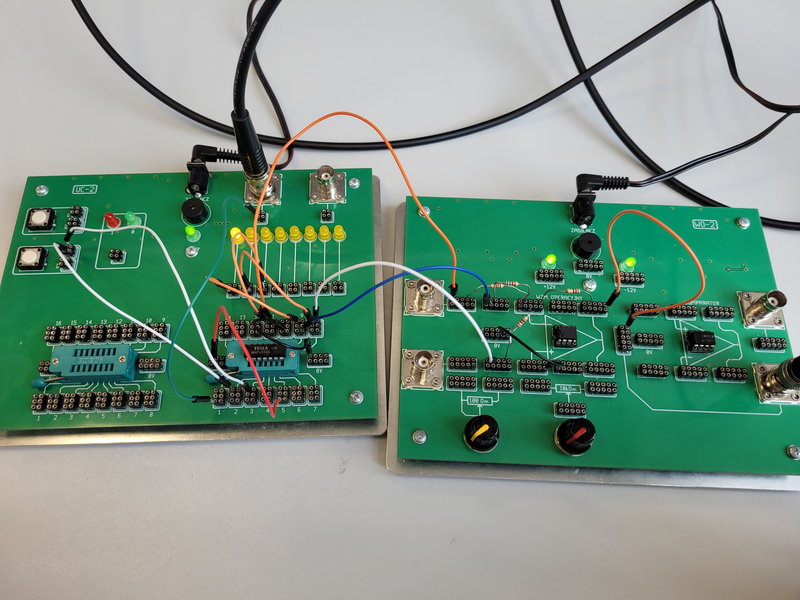
\includegraphics[width=\textwidth]{img/2/20220608_100038_scaled.png}
            \caption{Złożony układ z licznikiem i wzmacniaczem}
        \end{figure}
    \item Korzystając z oscyloskopu zaobserwowano napięcia wyjściowe z sumatora napięć.
        \begin{figure}[H]
            \centering
            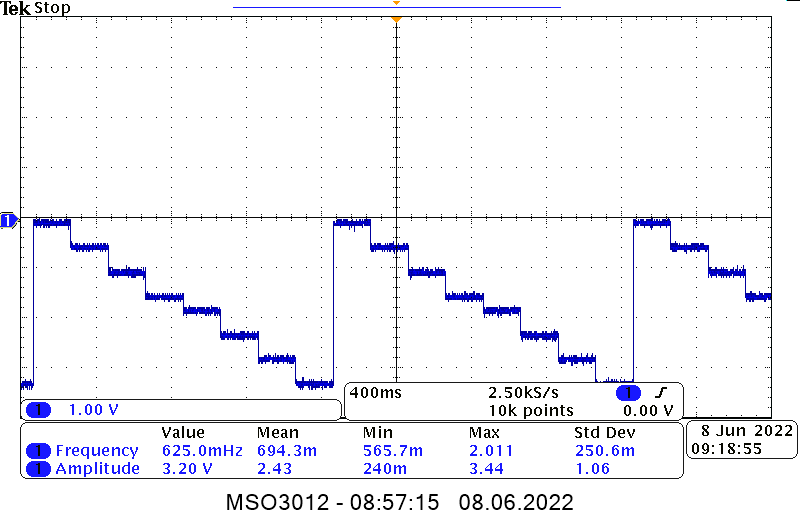
\includegraphics[width=\textwidth]{img/2/2_dziala2_cropped.png}
        \end{figure}
        Zaobserwowano 8 skoków w napięciu - dla każdego wskazania licznika binarnego, co zgadzało się z przewidywaniami.
    \item Układ działał poprawnie.
\end{itemize}